\documentclass[output=paper,colorlinks,citecolor=brown,modfonts,nonflat]{../langscibook}
\ChapterDOI{10.5281/zenodo.4032288}
\author{Heather E. Hilton\affiliation{Université Lumière Lyon 2}\orcid{}\lastand John Osborne\affiliation{Université Savoie Mont Blanc}\orcid{}}
\title{Analysing interaction in primary school language classes: Multilevel annotation and analysis with EXMARaLDA}
\abstract{Language classrooms provide a rich terrain for language acquisition research, and classroom observation has a long history (\citealt{Passy1885, Brebner1898})
% , including numerous studies of interaction within the foreign language class in the latter part of the 20\textsuperscript{th} century \citep{Véronique1992}.
This interest has resulted in a considerable set of transcribing conventions and observation grids%(\citealt{SinclairCoulthard1975, Moskowitz1976, AllenEtAl1983, UllmannGeva1984})
, but the analytical techniques have varied little since the initial conversation analyses of the 1970s and 1980s: transcription is often done without the aid of dedicated software and analyses are carried out by hand.

As part of an exploratory study of elementary school foreign language learning, a French research team observed two classes% (25 pupils in Year 1, 30 in Year 3, aged 6 and 8 respectively)
during their first year of beginning-level English lessons.
% Observation took place at three different times during the school year, with a total of three weeks of language lessons filmed in each classroom.

This chapter presents the methodology adopted for transcribing and annotating the lessons using EXMARaLDA (\citealt{SchmidtWörner2014})%, a tool which facilitates objective comparison of the two learning environments, and multi-level analyses.
% Our initial analyses illustrate
and analyzes
the ways in which well-designed transcription software can contribute to an understanding of methodological and interactional classroom variables, and how they may affect emergent language knowledge and skill in the classroom. Video-linked transcription and multi-tiered annotation in EXMARaLDA can enable automatic and semi-automatic analyses of various aspects of the classroom  experience%:  talking time, activity types, L1 and L2 use, teacher-learner and learner-learner interactions, metalinguistic input, visual input, manipulation of objects, and other actions.
Our analyses compare the two classrooms and explore features of these young learners’ initial contact with new words and their semantic-grammatical properties.

\keywords{early language learning, classroom interaction, transcription methodology, teaching methodology}
}
\IfFileExists{../localcommands.tex}{
  % add all extra packages you need to load to this file

\usepackage{tabularx,multicol}
\usepackage{url}
\urlstyle{same}

\usepackage{enumitem}

\usepackage{listings}
\lstset{basicstyle=\ttfamily,tabsize=2,breaklines=true}

\usepackage{langsci-basic}
\usepackage{./langsci-optional}
\usepackage{langsci-lgr}
\usepackage{langsci-gb4e}

\usepackage{jambox}

\newfontfamily\cjkfont
  [Scale=MatchLowercase,BoldFont=SourceHanSerifSC-Bold.otf]{SourceHanSerifSC-Regular.otf}
\AdditionalFontImprint{Source Han Serif}


\usepackage{siunitx}
\sisetup{output-decimal-marker={.},detect-weight=true, detect-family=true, detect-all, input-symbols={\%}, free-standing-units, input-open-uncertainty= , input-close-uncertainty= ,table-align-text-pre=false,uncertainty-separator={\,},group-digits=false,detect-inline-weight=math}
\DeclareSIUnit[number-unit-product={}]{\percent}{\%}
\makeatletter \def\new@fontshape{} \makeatother
\robustify\bfseries % For detect weight to work

  \newcommand*{\orcid}{}

\renewcommand{\sectref}[1]{Section~\ref{#1}}

% \renewcommand{\lsCoverTitleFont}[1]{\sffamily\addfontfeatures{Scale=MatchUppercase}\fontsize{41pt}{15mm}\selectfont #1}
% \renewcommand{\lsChapterFooterSize}{\scriptsize}

\makeatletter
\let\thetitle\@title
\let\theauthor\@author
\makeatother

\newcommand{\togglepaper}[1][0]{
%   \bibliography{../localbibliography}
  \papernote{\scriptsize\normalfont
    \theauthor.
    \thetitle.
    To appear in:
    Change Volume Editor \& in localcommands.tex
    Change volume title in localcommands.tex
    Berlin: Language Science Press. [preliminary page numbering]
  }
  \pagenumbering{roman}
  \setcounter{chapter}{#1}
  \addtocounter{chapter}{-1}
}

\newcommand{\keywords}[1]{\noindent\bfseries Keywords: \MakeCapital#1}

\let\oldtabularx\tabularx	% number in tabulars
    \let\endoldtabularx\endtabularx
    \renewenvironment{tabularx}{\normalfont\addfontfeatures{Numbers={Monospaced,Lining}}\selectfont\oldtabularx}{\endoldtabularx}


\newcommand{\NS}{\hphantom{N}{NS}:}
\newcommand{\TRS}{\hphantom{NNS:}~}
\newcommand{\NNS}{NNS:}
 
  %% hyphenation points for line breaks
%% Normally, automatic hyphenation in LaTeX is very good
%% If a word is mis-hyphenated, add it to this file
%%
%% add information to TeX file before \begin{document} with:
%% %% hyphenation points for line breaks
%% Normally, automatic hyphenation in LaTeX is very good
%% If a word is mis-hyphenated, add it to this file
%%
%% add information to TeX file before \begin{document} with:
%% %% hyphenation points for line breaks
%% Normally, automatic hyphenation in LaTeX is very good
%% If a word is mis-hyphenated, add it to this file
%%
%% add information to TeX file before \begin{document} with:
%% \include{localhyphenation}
\hyphenation{
affri-ca-te
affri-ca-tes 
Berg-green
Jap-a-nese
Gram-mat-i-cal-i-ty
Mac-Whin-ney
Lec-lercq
meth-od-o-log-i-cal
}

\hyphenation{
affri-ca-te
affri-ca-tes 
Berg-green
Jap-a-nese
Gram-mat-i-cal-i-ty
Mac-Whin-ney
Lec-lercq
meth-od-o-log-i-cal
}

\hyphenation{
affri-ca-te
affri-ca-tes 
Berg-green
Jap-a-nese
Gram-mat-i-cal-i-ty
Mac-Whin-ney
Lec-lercq
meth-od-o-log-i-cal
}
 
  \bibliography{../localbibliography}
  \togglepaper[1]%%chapternumber
}{}

\shorttitlerunninghead{Analysing interaction in primary school language classes}
\begin{document}
\maketitle
\vspace*{-3cm}~\newpage

\section{Introduction}

Classroom observation has a long history in the context of language teaching methodology and teacher training (see, for example, \citealt{Passy1885, Brebner1898}), and the language classroom became a valued research context for second language acquisition (SLA) and interaction research in the late 1960s (\citealt{Moskowitz1976, Jarvis1968, Wragg1970, SeligerLong1983, Allwright1984, Véronique1992}). Researchers were justifiably interested in observable factors that might influence the emergence of new language forms and structures, in learners of different ages and backgrounds. Since these early studies, interest in classroom interaction has remained steady, with particular attention paid to the interactions between learners as they work together in groups, or in computer-mediated “tandem” situations (for example, \citealt{DevelotteEtAl2008}). The authors of this paper are newcomers to interaction research, having previously carried out work on native-speaker and learner corpora generated through monological or guided tasks. Our previous transcription experience had been with the CHILDES suite of software \citep{MacWhinney2000} and the associated PHON software \citep{RoseEtAl2006}; we are firmly committed to Brian MacWhinney’s paradigm-changing stance on the need for shared data in language acquisition research \citep[27--30]{MacWhinney2010}.

With the objective, therefore, of taking a data-driven and data-sharing approach to the analysis of classroom interaction, this chapter will present our analyses of English as a Foreign Language  (EFL) lessons filmed in two primary schools in France. The rationale for choosing the EXMARaLDA software (\citealt{SchmidtWörner2014}) will be explained, as well as our transcription and annotation system. In the last two sections of the chapter, we will illustrate the types of analyses that can be carried out with a well-designed tool, and consider the potential of such analyses for research in second language acquisition and teaching.

\section{Classroom interaction research (theoretical and methodological issues)}\label{sec:hilton:2}

Early observations of classroom interaction (\citealt{Flanders1970,Brown1975,Moskowitz1976,Bowers1980,AllenEtAl1983,UllmannGeva1982, UllmannGeva1984}) led to various means of representing what was going on in the classroom, often using tables or checklists completed by hand in real time. These observation methods were generally developed for pedagogical purposes such as teacher training rather than being part of a concerted research programme, and resulted in a spate of introductory texts for language teachers at the end of the 1980s (\citealt{Allwright1988,Chaudron1988,Lier1988,Nunan1989}).

A notable exception, giving more attention to linguistic and pragmatic aspects of classroom exchanges, is the system developed by \citet{SinclairCoulthard1975} for describing the structure of classroom discourse. In one of the most detailed early studies of interaction in the EFL classroom, \citet{Willis1981} used a modified version of \citeauthor{SinclairCoulthard1975}’s system to analyse a corpus of tape-recorded lessons. The recordings were made with a double-track machine, with one microphone for the teacher and one for the learners. Non-linguistic and inaudible features were hand-noted along with the time-counter position on the tape-recorder. These data were then transcribed by hand in a multi-column format, indicating the structure of exchanges and the type of act. This resulted in a total of 27 categories, based on \citeauthor{SinclairCoulthard1975}’s initial inventory of: marker, starter, elicitation, check, directive, informative, prompt, clue, cue, bid, nomination, acknowledge, reply, react, comment, accept, evaluate, metastatement, conclusion, loop and aside. The descriptive categories developed in this framework, either as originally defined by \citeauthor{SinclairCoulthard1975} or in a modified form, have subsequently been used in a large number of analyses, notably those deriving from the postgraduate programme in Teaching English as a Foreign Language at Birmingham University, but also by researchers elsewhere (\citealt{Chaudron1977, GrandcolasSoulé-Susbielles1986, Chapelle1990}). They have been partly adapted for the present study.

Classroom interaction studies have also drawn on the techniques used in Conversation Analysis (CA) for describing naturally occurring speech. These include accounting for such things as turn-taking organization \citep{SacksEtAl1974}, repair (\citealt{SchegloffEtAl1977, Schegloff2000}), the cooperative nature of “side sequences” \citep{Jefferson1972} or discourse as “interactional achievement” \citep{Schegloff1982}, but also defining conventions for detailed transcription of interactions \citep{Jefferson2004}, including those where participants have non-targetlike discourse characteristics, as in the case of children \citep{Ochs1979} or L2 speakers (\citealt{Jefferson1983, Jefferson1996}). In second language acquisition (SLA) research, interest in using CA techniques was stimulated partly by criticism that SLA reflected an imbalance in favour of individual cognition at the expense of interactional and sociolinguistic orientations to language (\citealt{FirthWagner1997}). Whether or not one subscribes to \citeauthor{FirthWagner1997}’s arguments (for responses see \citealt{Kasper1997,Poulisse1997,Long1997,Gass1998}) there is no doubt that they triggered interest in applying CA to various kinds of SLA data (\citealt{Markee2000,Seedhouse2004, Seedhouse2005}) and in exploring the “intersection” between CA, SLA and language pedagogy \citep{Mori2007}. A more recent development is the convergence between CA methodology and complexity theory to investigate the ways in which L2 classroom interaction displays characteristics of a complex adaptive system (\citealt{Seedhouse2010, Seedhouse2015}).

With the advent of video recording it became no longer necessary to use checklists and annotations in real time since in principle all the data could be retrieved at leisure from the recording. However, as well as being more intrusive, filming necessarily imposes a frame on what is actually captured by the camera, and the subsequent transcription introduces a further filter determined by the transcription format and by what the transcriber chooses to pay attention to. Transcription is a selective process \citep{Ochs1979} and the transcript itself is an evolving flexible object \citep{Mondada2007}. Researchers often continued to use a play-script format ill-adapted to the complexity of video data (see \citealt{Erickson2004}). As \citet[17]{Jones2013} notes, “[t]he problem with most early work using video was that technologies of transcription had not yet caught up with the technologies of recording.” Dedicated software for multimodal transcription such as ELAN, EXMARaLDA or ANVIL (\sectref{sec:hilton:3.3} below) frees the transcriber from the constraints of a page format, facilitates the representation of overlaps, simultaneous events or non-linguistic features, and enables transcription segments to be time-linked to the digital recording. However, the raw data of the recording still have to go through a process of “entextualization” (\citealt{BaumanBriggs1990}) in order to be fully searchable, and it is the decisions made at this stage that will determine which aspects of the data can subsequently be retrieved for analysis. 

Searchability is an important condition, both for quantifying chosen features of classroom interaction and for examining elements that may be dispersed throughout a lesson. Studies of interaction in SLA, inside and outside the classroom, have often followed a path suggested by \citegen{Jefferson1972} notion of “side sequences” and have focused on instances of communicational problem solving and negotiation that are thought to have a potential for triggering acquisition, following work by \citet{PietroEtAl1989,Vasseur1989} and \citet{Bange1992}. The methodology of these studies consists largely of micro-analyses of interactions (\citealt[7]{Pekarek-Doehler2000}) and although it is emphasised that behind these analyses lies an entire corpus (\citealt[3]{ArdittyVasseur2005}), the data presented for discussion consist essentially of selected extracts. This is fair enough within a given research perspective – interested specifically, say, in interactional shifts of focus between communication and the means of communication – but it is also possible to adopt a more "corpus-driven" approach to classroom data, in which analysis is bottom-up and data-driven (\citealt{Tognini-Bonelli2001,Seedhouse2005}), with the aim of capturing patterns and associations that may not have been expected at the outset.

\section{Methodology of the current study}\label{sec:hilton:3}
\subsection{{The context}\label{sec:hilton:3.1}}

The \textit{Seine \& Marne Primary} project is an exploratory study by a multidisciplinary team of researchers, which was implemented between 2012 and 2015 in two public elementary schools in the Seine \& Marne département west of Paris, France. During the 2012--2013 school year, two classrooms of beginning English were filmed at three intervals: early December, mid-February, and mid-May. In one classroom, 25 children in their first year of primary school (15 girls and 10 boys, all born in 2006) were six years old at the time of filming; in the other, 29 Year 3 learners (16 girls and 13 boys, all born in 2004), were eight years old at the time of the study.\footnote{The research team was able to take advantage of a change in the national curriculum for foreign languages, which lowered the starting point for L2 study in 2011, and enabled this comparison of children starting English at age six, and age eight in the same school system during the 2012--2013 school year.} The two classrooms are in adjacent villages (two kilometres apart), part of a \textit{regroupement} \textit{scolaire}, or closely-linked network of rural schools, where the socio-economic composition of the classes is basically identical. Seven of the 54 children participating in the study are bilingual (users of a language other than French in their daily lives), according to language profile information provided by the parents (three children in Year 1, four in Year 3).

The institutional context of the \textit{Seine \& Marne Primary} study was a 2012 ruling by the French Ministry of Education to move obligatory foreign language tuition into the first year of primary school, despite problems of in-service and even initial teacher training for this aspect of the elementary curriculum (\citealt{YoungMary2010,Mary2014}). The French education system is highly centralized, with a national curriculum, so a common communicative task-based methodology (\citealt{CouncilofEurope2001}) is used in both classrooms: the syllabus is functionally-organized (greeting, asking and telling your name or age, expressing likes and dislikes, etc.) and classroom activities include small group work, interactional role plays, games and tasks (e.g., cooking, planting seeds). Both teachers use real objects and pictures to illustrate meaning (of new words, especially) and puppets to help trigger functional language. The Year 1 teacher created all of her support materials and used storybooks at the end of each lesson; the Year 3 teacher based her lessons on a commercially-available textbook, with an increasing number of self-designed activities throughout the year but no use of storybooks. Both the first- and third-year groups had 80 to 90 minutes of English per week, in keeping with the national curriculum, although this total was distributed differently throughout the week, with more frequent, shorter sessions in Year 1, and two 45-minute sessions in Year 3. A one-hour interview with each teacher early in the year revealed a key institutional variable: both teachers are highly confident and competent professionals (displaying detailed knowledge of the curriculum, their learners and family attitudes towards language-learning, as well an advanced level of methodological analysis), but they possess very different levels of \textit{linguistic} confidence, in relation to their obligatory English teaching. The Year 1 teacher majored in English at university, lived two years in the United States, and declared herself to be very comfortable (“\textit{très} \textit{à} \textit{l’aise}”) with the foreign-language part of her curriculum. The Year 3 teacher majored in Economics and volunteered to participate in the project precisely because she wanted help with her English lessons, feeling quite uncomfortable with her knowledge of the language (“\textit{tellement} \textit{pas} \textit{à} \textit{l’aise}”), in particular of English pronunciation and grammar. \sectref{sec:hilton:4} below will discuss whether this difference in linguistic confidence may be reflected in the methodological or linguistic characteristics of each teacher’s pedagogical approach and, as a consequence, in general classroom organization.

\subsection{{Overall study design and research questions}\label{sec:hilton:3.2}}

In the context of newly-imposed foreign language lessons in Year 1, the objectives of the \textit{Seine \& Marne Primary} \textit{Project} were wide-ranging and exploratory, attempting to answer research questions as varied as: What sort of language-teaching methodology is used in primary English classrooms in France? Are there differences in the methodology used with six-year-olds and with eight-year-olds, and if so, of what types? Do six- and eight-year-olds follow similar learning trajectories in the FL classroom, or are there fundamental differences? What role do individual variables (such as first-language knowledge, personality, cognitive capacity, motivation) play in the learning pathways observed? 

In order to answer these questions, three data sets were collected: the video corpus of 14 filmed lessons, the children’s performance on a series of English tasks (measuring emergent knowledge and skill and administered twice during the 2012--2013 school year), and their scores on a battery of psychometric measures of cognitive and social characteristics. The linguistic and psychometric data have been discussed in other studies (\citealt{HiltonRoyer2014, HiltonEtAl2016, Hilton2017}). In this chapter we will be presenting the methodology used to transcribe and annotate the filmed language lessons, as well as the types of classroom analyses that such an approach makes possible. The precise questions for this study are as follows:

\begin{itemize}
\item To what extent can carefully transcribed and annotated language lessons shed light on classroom foreign-language teaching and learning processes?
\item Which automatic analyses (enabled by the transcription software) are revealing of classroom interactions?
\item Which additional analyses can add information on classroom interaction structures?
\end{itemize}
\begin{itemize}
\item What types of conclusions for language-learning and teaching research can be drawn from such analyses?
\end{itemize}

To film the 14 lessons comprising our video corpus, a single Canon XF100 video camera was used (at times fixed to a tripod, at times roving and zooming in on the children); the teachers wore a cordless lapel microphone during the lessons, and a boom-held microphone (which could follow the sound around the room, for example during group work) was also used for an optimal sound feed. The corpus of filmed lessons was assembled in order to gather information on lesson content and a concrete sample of the types of classroom activities used, for a more complete picture of the children’s learning environment. The data obtained are very sparse (six to eight lessons out of an annual program), and the use of a single camera (focusing alternatively on the teacher or the learners) means that the footage obtained cannot be used for detailed observation of the classroom behaviour of each child. For this methodologically-oriented chapter, we will focus our analyses here on the two most similar lessons from our classroom corpus: both occurring in mid-February and both devoted to the presentation and practice of new food vocabulary in a unit devoted to talking about food, preferences, and cooking.

\subsection{{Choice of transcription software}\label{sec:hilton:3.3}}

When choosing a transcription tool, the guiding criterion should be the fit between the objectives of the study and what the transcription software is designed to do. To transcribe and analyse the lessons in the \textit{Seine \&  Marne} project, our primary focus was classroom interaction and methodology: teacher talking time, learner talking time, language use (L2 English or L1 French), the linguistic content of teacher and learner productions, the different types of interactions between teacher and learner(s), and the typology of classroom activities and teaching techniques. It therefore seemed logical to adopt software designed precisely for the annotation of interactive discourse. 

Several freely available scientific tools can be used, most notably CLAN \citep{MacWhinney2000}, ANVIL \citep{Kipp2014}, ELAN \citep{WittenburgEtAl2006} and EXMARaLDA (\citealt{SchmidtWörner2014}). Others, such as the \textit{Digital} \textit{Replay} \textit{System} \citep{BrundellEtAl2008}, offer interesting features but are no longer supported. The most apparent difference between tools, from the transcriber’s point of view, is whether they display discourse as a list of turns (as in CLAN) or in tiers of timelines (as in ELAN or EXMARaLDA). According to the purpose for which they have been designed – CLAN for morpho-syntactic and lexical analyses in child language, PHON for finer phonological transcriptions of emergent child speech, ELAN for easier coding of non-verbal phenomena in linguistic studies (\citealt{LausbergSloetjes2009}) – each tool has slightly different ways of setting up transcription tiers and incorporates different sub-programmes for segmentation and automatic pause recognition, concordancing, morpho-syntactic tagging, lexical analysis, etc. With the most widely-used tools, import and export from and to the other formats is possible, if not always lossless, so choice of a particular tool does not lock the user irrevocably into that environment. For an extensive overview of tools for multimodal annotation and interactional analysis see \citet{CassidySchmidt2017} and \citet{Glüer2018}.

The choice of EXMARaLDA, developed by Thomas Schmidt, Kai Wörner, Timm Lehmberg and Hanna Hedeland at the \textit{Zentrum} \textit{für} \textit{Sprachkorpora} at Hamburg University (\citealt{SchmidtWörner2014}), was determined by its tier-timeline format (more suitable for classroom interaction than a list of turns), by its ability to handle multi-level concordancing through the built-in EXAKT tool, and by what appeared, after initial tests with ELAN, to be a more flexible way of setting up transcription and annotation tiers for multiple speakers. However, we have no reason to suppose that the annotations and analyses discussed here could not also be carried out with ELAN, with a slightly different procedure for determining tier types. As with any multimedia software, ability to read video formats can be an issue. EXMARaLDA recommends mpeg4 for video files and wav for audio, and incorporates four different media players to choose from for the best compatibility.

\subsection{{{\textit{Seine \&}} {\textit{Marne}} transcription architecture and annotation conventions}\label{sec:hilton:3.4}}

Because of the use of a single camera for filming the \textit{Seine \& Marne Primary} English lessons, we limited our transcription architecture to three primary speaker transcription tiers: Teacher, Learner-groups, and Individual learner. The “Learner-groups” line was used to transcribe any learner productions involving two or more children (with specifications concerning group size in a dependent tier); the “Individual learner” line was used to transcribe any production by an individual child (again, with individual learner characteristics (sex, project ID number) given in a dependent tier, whenever possible, our single-camera installation making it impossible to identify the source of every utterance). In order to facilitate automatic word-counts in EXMARaLDA and subsequent concordancing operations, we created two transcription lines for each speaker, one for productions in L2 English, and one for productions in L1 French. Three dependent tiers are attached to each speaker: one for the fixed coding of the interactional function of each transcribed segment, using the set of codes described in \tabref{tab:hilton:1}, an open tier for annotating any relevant or salient actions, and a tier for fixed coding of linguistic errors (selection from the list of codes). Additional independent tiers are used to annotate activity types, lesson plan structure, and support material used; a “comments” line enables the transcriber to note anything else of interest. A particularly transcriber-friendly aspect of EXMARaLDA is the possibility of formatting the transcription lines with colour-coding, for example, so that all tiers linked to the same speaker have the same background colour.

Classroom speech turns are lexically (and not phonologically) transcribed for each speaker, using a simplified version of basic CHAT transcription conventions (Codes for the Human Analysis of Transcripts, \citealt{MacWhinney2000}), which the \textit{Seine \&} \textit{Marne} research team had already used extensively. An example of the transcription output from EXMARaLDA is shown in \figref{fig:hilton:1}. The transcription format uses the following basic units:

An \textit{interval} is a portion of the time-line in EXMARaLDA and is typically the duration occupied by a single consecutive event (see below). Intervals are numbered consecutively from the beginning to the end of the recording, as shown in the top bar in \figref{fig:hilton:1}.

An \textit{event} is a portion of the transcription, and can be either a speech event, containing speech by one of the speakers, or a classroom event, corresponding to an action with or without transcribed speech attached to it. Thus in \figref{fig:hilton:1}, there are five speech events (respectively “oh!”, “now”, “look and listen very carefully”, “okay?” and “okay”) and four classroom events. One of these (“gesturing...”) accompanies a speech event by the same participant, one (“changing file”) coincides with a speech event by other participants, and two are unaccompanied by any speech (“returning to seat” and “pointing to picture”).

An \textit{utterance} can consist of a single word, a verbless phrase or a main clause with any of its dependent clauses. Typically, an utterance will correspond to a speech event, but utterances containing more than one interactional function (\tabref{tab:hilton:1}, below) are broken down according to these functions. For example, “Martin {\textbar} sit down please” counts as two EXMARaLDA speech events, the first one nominative, the second directive.

A \textit{segment} \textit{chain} is an interrupted string of speech by one speaker (i.e., a speech turn) and can consist of one or more utterances. The “output” command in EXMARaLDA can be used to generate the transcription as a list of turns, with each segment chain on a separate line.

The EXMARaLDA Annotation Panel was used to simplify the coding of the interactional function of each segment, with a fixed set of codes based on \citeapo{Willis1981} modified version of \citegen{SinclairCoulthard1975} interaction typology (see \sectref{sec:hilton:2}, above). We pared the system down further, to correspond to the particular types of interaction found in these beginning-level primary classrooms. \tabref{tab:hilton:1} presents the 29 codes used to annotate interactional behaviours in our corpus, grouped in eleven interactional functions. The Annotation Panel enables the transcriber to insert the relevant code on the interaction tier for each speech event or interval, without typing it out each time.

\begin{table}
\caption{Coding system used to annotate classroom interactions\label{tab:hilton:1}}
\footnotesize
\begin{tabularx}{\textwidth}{llQ}
\lsptoprule
&  Interaction &  Explanation\\
&  type, codes & \\\midrule
 1 & meta            & comment on lesson structure, activity, language\\
   &  metaPRE        & PRE: prior to activity or lesson (statement of objectives; beginning of new lesson phase)\\
   &  meta MID       & MID: explaining, commenting on something as it is happening (during activity)\\
   &  metaPOST       & POST: summing up \& analyzing; marking end of episode/activity\\
   &  metaCHECK      & CHECK: checking comprehension, uptake\\\midrule                              
 2 & aside           & elements of discourse not intended to elicit response or reaction (teacher “thinking out loud”, talking to self or film crew…)\\\midrule
 3 & directive       & request nonlinguistic response; classroom management\\\midrule
 4 & presentation    & declarative statement, presentation\\
     & presLANG       & of sound, word, structure (even question)\\
     & presCULT       & of cultural information\\
     & presMOD        & of model for student production/repetition\\
     & presINFO       & of general information (about something other than above) \\\midrule
 5 & elicitation     & request\slash elicit response\\
      & elicitS        & with a statement\\
      & elicitQ        & with a question\\
      & elicitNV       & non-verbal elicitation\\
      & elicitPROMPT   & reiterate stalled elicitation, give a clue, etc.\\
      & elicit\_REP    & elicit a repetition\\
      & elicit\_CORR   & elicit a correction\\\midrule
 6 & nomination & call on a learner, give permission to respond\\\midrule
 7 & acknowledgement            & acknowledge a response, accept a bid\\
     & ack       & positive acknowledgement, indicate appropriate response\\
     & ackNEG    & indicate that response or reaction is inappropriate\slash incorrect\\\midrule
 8 & response           & provide linguistic response to elicitation or prompt\\
        & resp          & (any response not in the following categories)\\
        & respANS       & answer (in response to a question)\\
        & respN         & naming (a picture or object, in response to non-verbal elicitation)\\
        & respREP       & repetition (repeating elicitation, with no change)\\
        & respRFORM     & reformulation (of preceding response; one or more changes; does not have to be by same speaker)\\
        & respCORR      & provide a correction (does not have to be by same speaker)\\\midrule
9 & {production} & spontaneous production (does not follow elicitation)\\\midrule
 10 & {reaction} & nonlinguistic response to directive or elicitation\\\midrule
 11 & {bid} & signal a desire to contribute \\
\lspbottomrule
\end{tabularx}
\end{table}

Linguistic errors were coded according to a minimalistic version of the error codes used in the PAROLE corpus \citep{Hilton2008}, which are based on error codes established for CHAT. An “error” is any divergence from expected forms in pronunciation, morphology, syntax or lexis (and no value judgment is placed on the use of this term, of course).



\figref{fig:hilton:1} shows the partition-formatted html output for seven intervals in the Year 3 lesson: transcription tiers are indicated in black headings and the dependent tiers in light grey; the partition illustrates the use of colours to link annotations to the relevant speaker.

\begin{figure}[b]
\caption{Partition-format output of finished transcription\label{fig:hilton:1}}
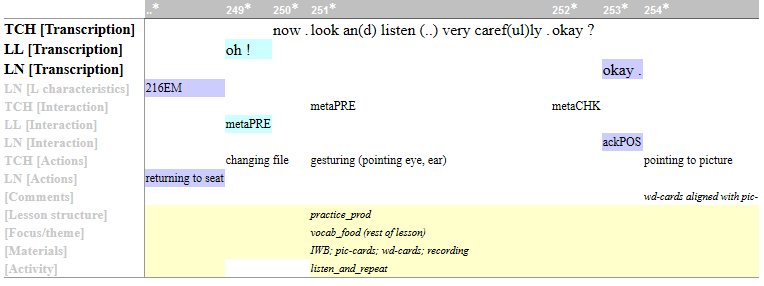
\includegraphics[width=\textwidth]{figures/hilton-img001.png}
\end{figure}
 
This easily-obtained output format is useful for checking transcriptions (only tiers containing transcription or annotation are shown in each partition) and for subsequent qualitative analysis.

\section{Analyses and preliminary findings} \label{sec:hilton:4}

Once the transcriptions are finalised, it is possible to carry out a number of analyses automatically – with pre-programmed functions in EXMARaLDA (section 4.1) – and semi-automatically – using the EXMARaLDA concordancing software, EXAKT (section 4.2). It is also easy to export EXMARaLDA files into a format enabling the use of the many powerful language-analysis programmes included in CLAN, but we will not have space to present these here.

\subsection{{Classroom comparisons through automatic analyses}}\label{sec:hilton:4.1}

Our first automatic tally concerns the number of transcribed \textit{segments}: a segment (more specifically,  in EXMARaLDA terminology, a \textit{segment chain}) corresponds to a speech turn, or uninterrupted string of speech by one speaker, which may contain more than one utterance. For example, \figref{fig:hilton:1} shows one segment by the teacher (“now. look an(d) listen (…) very caref(ul)ly. okay?”) covering intervals 250--252, bounded on either side by a learner segment (“oh” and “okay”, respectively). Speaker-specific segment counts are obtained with a single click in EXMARaLDA, and are presented in \tabref{tab:hilton:2}, below. These figures illustrate the intense interactional nature of the beginning language classroom, with around 20 speech turns per minute in both classrooms – that is, one every three seconds.

\begin{table}[b]

\caption{Number of segments for each speaker (columns) per classroom (lines)\label{tab:hilton:2}}
\small
\begin{tabular}{l >{\centering}p{2cm} >{\centering}p{2cm} >{\centering}p{2cm} c  >{\centering}p{3cm}@{}c}
\lsptoprule
& {\raggedright Teacher}\newline (+~recordings) & Learner-group & Individual learner & ~\newline Total & Speaking turns\newline per minute &\\
 \midrule
Year 1\footnote{41-minute  lesson.} & 369 & 306 & 188 & 863 & 21 &\\
Year 3\footnote{43-minute  lesson. The Year 3 lesson includes ten pre-recorded one-word utterances.} & 404 & 223 & 239 & 866 & 20 &\\
\lspbottomrule
\end{tabular}
\end{table}

As with most audio- or video-linked transcription software, it is easy in EXMARaLDA to obtain a calculation of speaking time for each of the transcription tiers: in other words (for the transcription architecture presented here) total teacher speaking time, and total learner speaking time, subdivided into learner-group and individual-learner speaking time. \figref{fig:hilton:2} illustrates the distribution of talking time in our two target lessons, with slightly more teacher talking time (the darker sectors on the right of each pie chart) in the Year 1 classroom, and both teachers (plus 0.4\% pre-recorded sound files in Year 3) occupying about half of the lesson time. The charts illustrate an interesting difference in learner participation in the two classrooms, with the Year 1 teacher eliciting more learner-group productions, and the Year 3 classroom characterised by more frequent individual learner productions.

\begin{figure}
\caption{\label{fig:hilton:2}Distribution of classroom talking time}
    \begin{tikzpicture}
    \pie[radius=2,color={silptwo,silpthree,silpfour},rotate=90]{15/~, 31/~, 54/~}
    \pie[radius=2,color={silptwo,silpthree,silpfour},text=legend,rotate=90,pos={5,0}]{25/learners-indiv, 27/learners-gp, 48/teacher}
    \node at (0,-2.5) {Year 1};
    \node at (5,-2.5) {Year 3};
    \end{tikzpicture}
% 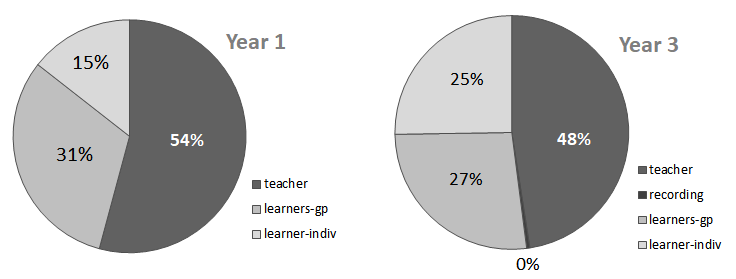
\includegraphics[width=\textwidth]{figures/hilton-img002.png}
\end{figure}

Our separate transcription lines for speech turns in L2 English or L1 French enable an automatic breakdown of the numbers of segments and words produced in each of the classroom languages; \figref{fig:hilton:3} gives a graphic presentation of the distribution of language use, based on the numbers of segments produced in each language. In both classrooms, at least 80\% of the teacher’s output is in English, with 92\% for the linguistically-confident Year 1 teacher; there is a higher percentage of English use overall in her classroom, particularly in the learners’ output. The unpruned data presented here includes asides and comments by the learners in L1 French; in both classrooms the inclusion of a food-tasting activity generated much excitement and a certain amount of L1 commentary. Both teachers carried out a metalinguistic wrap-up in French at the end of the lesson, and the Year 3 learners also had a short cultural discussion in French early in the lesson.

\begin{figure}[p]
\caption{\label{fig:hilton:3}Use of L2 English and L1 French by classroom and speaker}

    \begin{tikzpicture}
        \begin{axis}[
            width  = .8\textwidth,
            height = .45\textheight,
            symbolic y coords={
                \,learners-indiv,
                \,learners-gp,
                teacher+rec,
                ~,
                learners-indiv,
                learners-gp,
                teacher
            },
            axis lines*=left,
            bar width = 15pt,
            axis on top,
            xmajorgrids,
%             tick align=inside,
%             major grid style={draw=white},
            xbar stacked,
            xmin=0,
            xmax=100,
            ytick=data,
            ylabel style={yshift=1.4cm},
%             enlarge y limits={.5},
            ylabel={{Year 3\hspace{3cm}Year 1}},
            legend style={at={(1,.5)},anchor=east},
            legend columns=2,
%             enlarge x limits = false
        ]
        \addplot+[silptwo] plot coordinates {
            (59.8326359832636,\,learners-indiv)
            (49.7757847533632,\,learners-gp)
            (83.1683168316832,teacher+rec)
            (69.1489361702128,learners-indiv)
            (74.1830065359477,learners-gp)
            (92.1409214092141,teacher)
        };
        \addplot+[silpfour] plot coordinates {
            (40.1673640167364,\,learners-indiv)
            (50.2242152466368,\,learners-gp)
            (16.8316831683168,teacher+rec)
            (30.8510638297872,learners-indiv)
            (25.8169934640523,learners-gp)
            (7.85907859078591,teacher)
        };
        \legend{English,French}

%         \coordinate (A) at (axis cs:teacher,10);
%         \coordinate (B) at (axis cs:teacher,90);
%         \draw [black,sharp plot] (A) -- (B);
        \end{axis}
    \end{tikzpicture}
% learner-indiv
% learners-gp
% teacher + rec
% learner-indiv
% learners-gp
% teacher
%
% 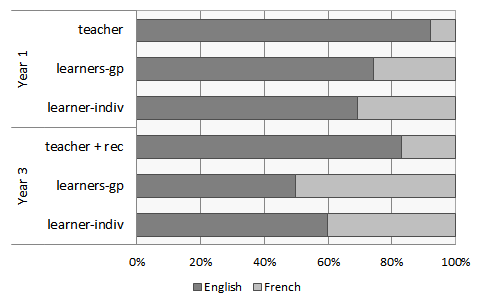
\includegraphics[width=\textwidth]{figures/hilton-img003.png}
\end{figure}
 


\begin{table}[p]
\caption{Numbers of words produced (unpruned tokens), by speaker and class\label{tab:hilton:3}}
\begin{tabular}{ll *{2}{S[table-format=4] S[table-format=1.1]}}
\lsptoprule
&  & \multicolumn{2}{c}{Year 1} & \multicolumn{2}{c}{Year 3}\\\cmidrule(lr){3-4}\cmidrule(lr){5-6}
&   &  {tokens} &  {wps\footnote{words per segment}} &  {tokens} &  {wps}\\
\midrule
 L2 English & teacher & \shadecell 2266 & 6.7 & 1206 & 3.7\\
& recording & {--} & {--} & 10 & 1.0\\
& learner groups &\shadecell 458 & 2.0 & 159 & 1.4\\
& indiv learner & 272 & 2.1 & 299 & 2.1\\
\tablevspace
 L1 French & teacher & 401 & 13.8 &\shadecell 703 & 10.3\\
& learner groups & 129 &  & 150 & \\
& indiv learner & 157 &  & \shadecell 462 & \\
\lspbottomrule
\end{tabular}
\end{table}


Before running the transcriptions through EXMARaLDA’s \MakeUppercase{Exakt} concordancing software, we can generate an unpruned word count, which enables a final automatic comparison between the two classrooms. \tabref{tab:hilton:3} shows additional characteristics of the two classrooms, with longer utterances in L1 French (unsurprisingly) in both classrooms, but also some interesting linguistic differences between the two classrooms (highlighted in grey). Learners in the Year 1 classroom heard almost twice as many English words during their 41-minute lesson as the Year 3 learners; despite their younger age, their English input also consists of longer L2 utterances (over six words per segment on average). The younger learners’ English output is also greater (in number of words produced), with slightly longer utterances in choral/group productions. The Year 3 learners produce more individual segments in L1 French than they do in English; many of these are comments on the new vocabulary words, or on the food-tasting activity.

These analyses, derived from a one-click count of transcription segments and timeline intervals, already point to linguistic and methodological differences between the Year 1 and Year 3 lessons. In the next section we will look more closely at the methodological, interactional, and linguistic characteristics of each classroom, using various concordancing options included in the EXMARaLDA package.

\subsection{{Classroom comparisons through further analyses}}\label{sec:hilton:4.2}

Using EXMARaLDA’s EXAKT concordancing programme, it is possible to pursue the comparisons between our two primary English classrooms. EXAKT enables the researcher to tally annotation codes on the dependent tiers according to speaker, to look at (and compare) the linguistic environment of target words or forms, and to carry out multi-tier analyses, combining a key word search on the transcription lines with information from the annotation tiers.

To compare the interactional patterns in our two lessons, we performed a simple count of the annotation codes on the "interaction" coding tiers, after filtering out the L1 transcription lines. Results are given here for patterns directly related to teacher-learner interaction: directives, modelling, elicitation, response and acknowledgement. Asides and metastatements, often in French, are not included. \figref{fig:hilton:4} shows interaction types in English in Year 1 and Year 3 for the teachers; \figref{fig:hilton:5} compares learner interaction in the two classrooms (where both individual and learner-group interactions have been combined). See \tabref{tab:hilton:1} above for an explanation of the interaction codes that are featured on the left of each chart.

\begin{figure}
% 	         ackNEG	ackPOS	directive	nomination	elicit_CORR	elicit_REP	elicitPROMPT	elicitQ	elicitS	presMOD
% Year 1	10	124	206	        69	         4	          1	          23	         68	5	98
% Year 3	15	75	74	      68	         10	         32	         50	         46	29	35

\hspace*{22mm}%
\begin{tikzpicture}[trim axis right,trim axis left]
    \begin{axis}[
        axis lines*=left,
        width  = .9\textwidth,
        height  = .6\textheight,
%         nodes near coords,
        ytick=data,
        y tick label style={},
        xbar,
        xmajorgrids,
        bar width=.3cm,
        xmin=0,
        legend style={at={(1,0.01)},anchor=south east},
        reverse legend,
        symbolic y coords={ackNEG,ackPOS,directive,nomination,elicit\_CORR,elicit\_REP,elicitPROMPT,elicitQ,elicitS,presMOD},
        ]
        \addplot[xbar,silptwo!80!black,fill=silptwo] plot coordinates {
            (98,presMOD)
            (5,elicitS)
            (68,elicitQ)
            (23,elicitPROMPT)
            (1,elicit\_REP)
            (4,elicit\_CORR)
            (69,nomination)
            (206,directive)
            (124,ackPOS)
            (10,ackNEG)
            };
        \addplot[xbar,silpfour!80!black,fill=silpfour] plot coordinates {
            (35,presMOD)
            (29,elicitS)
            (46,elicitQ)
            (50,elicitPROMPT)
            (32,elicit\_REP)
            (10,elicit\_CORR)
            (68,nomination)
            (74,directive)
            (75,ackPOS)
            (15,ackNEG)
            };
        \legend{Year 1, Year 3}
    \end{axis}
\end{tikzpicture}
    \caption{\label{fig:hilton:4}Teacher L2 interaction types, by classroom}
% 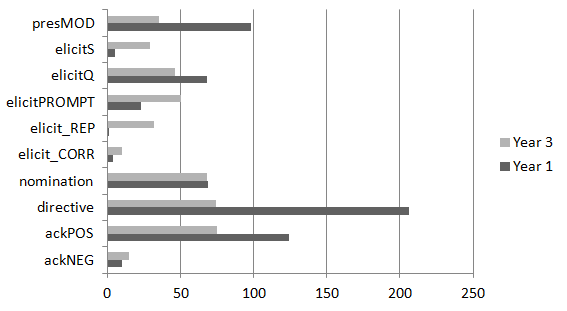
\includegraphics[width=\textwidth]{figures/hilton-img004.png}
 \end{figure}


 \begin{figure}
\hspace*{22mm}%
 \begin{tikzpicture}[trim axis right,trim axis left]
    \begin{axis}[
        axis lines*=left,
        width  = .9\textwidth,
        height  = .4\textheight,
%         nodes near coords,
        ytick=data,
        y tick label style={},
        xbar,
        xmajorgrids,
        bar width=.3cm,
        xmin=0,
        legend style={at={(1,0.01)},anchor=south east},
        reverse legend,
        symbolic y coords={reaction,respANS,respN,respREP,respRFORM,respCORR}
        ]
        \addplot[xbar,silptwo!80!black,fill=silptwo] plot coordinates {
            (74,reaction)
            (70,respANS)
            (46,respN)
            (130,respREP)
            (2,respRFORM)
            (1,respCORR)
            };
        \addplot[xbar,silpfour!80!black,fill=silpfour] plot coordinates {
            (26,reaction)
            (64,respANS)
            (1,respN)
            (91,respREP)
            (6,respRFORM)
            (6,respCORR)
            };
        \legend{Year 1, Year 3}
    \end{axis}
\end{tikzpicture}

% 	reaction	respANS	respN	respREP	respRFORM	respCORR
% Year 1	74	70	46	130	2	1
% Year 3	26	64	1	91	6	6
 \caption{\label{fig:hilton:5}Learner L2 interaction types, by classroom}
% 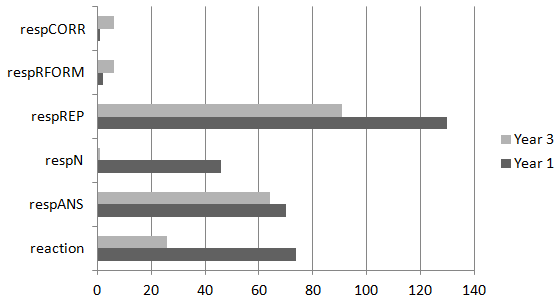
\includegraphics[width=\textwidth]{figures/hilton-img005.png}
 \end{figure}

The primary interactional difference between the two classes lies in the number of directives and of models for student production or repetition (coded presMOD) produced by the Year 1 teacher (\figref{fig:hilton:4}), and the (correspondingly) high proportion of naming responses (respN) produced by the Year 1 learners (\figref{fig:hilton:5}), as well as more repetition (respREP). In turn, these trigger a greater number of positive acknowledgements from the teacher.

The concordancing functions of EXAKT enable us to take a closer look at the linguistic contexts in which the new words appear in the two classrooms, and to compare the ways in which the two groups of learners structure utterances containing them. As the two lessons under examination here had food as the main topic, we are going to focus here on words related to this semantic domain.  

The list of L1 and L2 food words occurring in the two lessons, obtained from a simple word-count in EXAKT, is as follows:

\begin{description}[font=\normalfont]
\item[Year 1:]
 \begin{description}[font=\normalfont,noitemsep]
 \item[]
 \item[L2 words:] \textit{apple}, \textit{banana}, \textit{chicken}, \textit{chocolate}, \textit{egg}, \textit{fish}, \textit{ice-cream}, \textit{orange}, \textit{pea}, \textit{pear}, \textit{soup}, \textit{spaghetti}, \textit{string-beans}; 
 \item[L2 associated words which do not designate types of food:] \textit{food}, \textit{eat}, \textit{hungry}, \textit{mouth}; 
 \item[L1 words:] \textit{chocolat}; 
 \item[L1 associated words:] \textit{assiette}, \textit{déjeuner}, \textit{nourriture}, \textit{aliments}.
 \end{description}
\item[Year 3:]
 \begin{description}[font=\normalfont,noitemsep]
 \item[]
 \item[L2 words:] \textit{butter}, \textit{cake}, \textit{egg(s)}, \textit{flour}, \textit{lemon}, \textit{milk}, \textit{pancake(s)}, \textit{sugar}; 
 \item[L2 associated words:] \textit{eat}, \textit{taste}; 
 \item[L1 words:] \textit{beurre}, \textit{citron}, \textit{crêpe(s)}, \textit{farine}, \textit{lait}, \textit{oeufs}, \textit{sucre}; 
 \item[L1 associated words:] \textit{casserole}, \textit{cuisiner}, \textit{goûter}, \textit{ingrédients}, \textit{recette}.
 \end{description}
\end{description}
In the Year 3 class, each of the L2 food words, with the exception of \textit{cake} (which occurs only once) is accompanied by an L1 equivalent, whereas in the Year 1 class, this is the case for only one word, \textit{chocolate}. In both classes, occurrences of the target vocabulary items are distributed throughout the lesson, but in slightly different ways, as shown in \figref{fig:hilton:6} and \figref{fig:hilton:7}. The numbers on the horizontal axis indicate the position of occurrences during the lesson, with reference to the interval on the time-line in which they appear (in total, 1200 to 1300 intervals per 40-minute lesson, shown on the X axis in \figref{fig:hilton:6} and \figref{fig:hilton:7}).

\begin{figure}
\caption{\label{fig:hilton:6}Distribution of food words in Year 1 class}
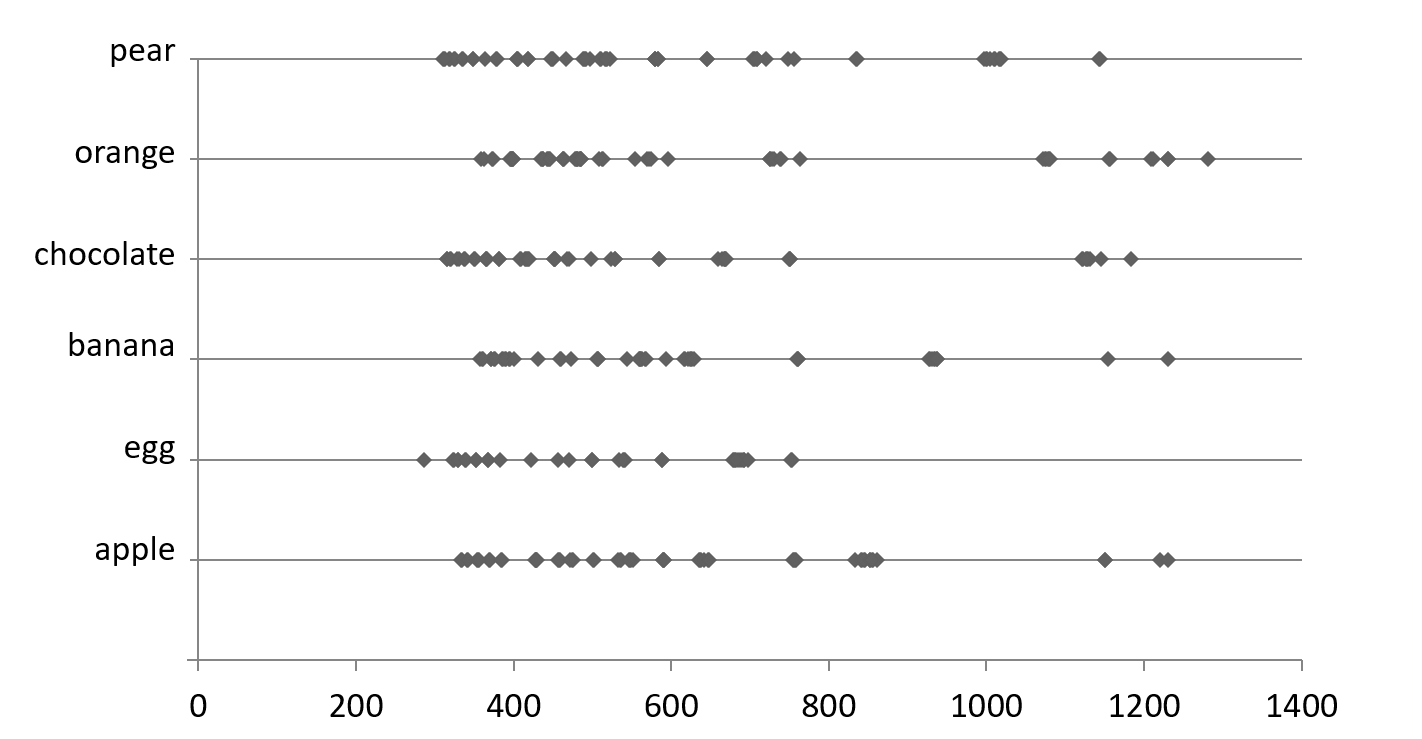
\includegraphics[width=\textwidth]{figures/hilton-img006.png}
\end{figure}
 

In the Year 1 class (\figref{fig:hilton:6}) there is an intensive repetition of all the target vocabulary in the first third of the lesson, followed by re-use of all the items except \textit{egg} towards the end of the lesson. In the Year 3 class (\figref{fig:hilton:7}), there are shorter bursts of repetition for some of the words – \textit{pancake,} \textit{egg,} \textit{flour,} \textit{milk} and \textit{butter}~– at slightly different moments, but otherwise the words are more randomly distributed between the beginning and the end of the lesson.

\begin{figure}
\caption{\label{fig:hilton:7}Distribution of food words in Year 3 class}
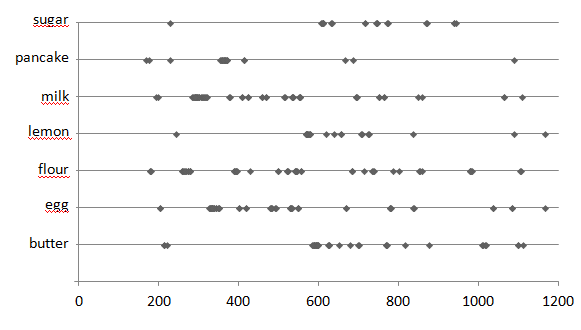
\includegraphics[width=\textwidth]{figures/hilton-img007.png}
\end{figure}
 

Appropriate use of food words in a complete English noun phrase depends partly on an appreciation of the mass-count distinction, since many foods can be presented and referred to either as substance or discrete units, often along a cline. The word \textit{chocolate}, for instance, can refer to individually wrapped chocolates, to a bar of chocolate, to cocoa, etc. – with consequences on its co-occurrence with determiners (\textit{∅}, \textit{a}, \textit{the}), with plural \textit{{}-s} and with singular or plural verb forms. Consequently, learners have to discover how to map particular determiner+noun+verb combinations onto their possible meanings. Potentially, various types of information are available to them: linguistic exemplars, feedback on their own productions, metalinguistic input, L1 analogies, word-referent associations and physical contact. To what extent are these different kinds of information present in classroom interaction, how do they combine, how do they vary from one class to the other, and with what result on the language of the learners themselves? Contextual information about these occurrences can be obtained with EXAKT, which as a first step displays basic key-word-in-context (KWIC) concordance lines, listed by speaker and by order of occurrence. \figref{tabfig:hilton:8} shows a concordance for the word \textit{apple} as used by the teacher in the Year 1 class, in order of occurrence.


\begin{figure}
\caption{\label{tabfig:hilton:8}KWIC concordance for {\textit{apple}},  {Year}  {1}  {teacher}}
\fittable{
\footnotesize\ttfamily
\begin{tabular}{l@{}l@{}lr@{~}l@{~}l}
\lsptoprule
% & %\textbf{Comm}  %Is this column needed?
% &   &  &  & \\
% \midrule
 \textbf{1} &  &  &  & \textbf{apple} & .\\
 \textbf{2} &  &  &  & \textbf{apple} & .\\
 \textbf{3} &  &  &  & \textbf{apple} & . \\
 \textbf{4} &  &  &  & \textbf{apple} & . \\
 \textbf{5} &  &  &  & \textbf{apple} & .\\
 \textbf{6} &  &  &  & \textbf{apple} & .\\
 \textbf{7} &  &  &  & \textbf{apple} & . \\
 \textbf{8} &  &  &  is it (..) [*] & \textbf{apple} & ? \\
 \textbf{9} &  &  &  is it & \textbf{apple} & ? no: .it 's not apple what is it ? \\
 \textbf{10} &  & &  is it apple ? no: .it 's not & \textbf{apple} & what is it ? \\
 \textbf{11} &  & &  it 's an & \textbf{apple} & . is it an apple ? ye:s . it 's an appl\\
 \textbf{12} &  & &  it 's an apple . is it an & \textbf{apple} & ? ye:s . it 's an apple . very good . \\
 \textbf{13} &  & &  apple . is it an apple ? ye:s . it 's an & \textbf{apple} & . very good . \\
 \textbf{14} &  & &  it 's an & \textbf{apple} & .what is it ? \\
 \textbf{15} &  & &  ybody on your board you [*] draw (..) an & \textbf{apple} & . [/] you draw an apple . on your board\\
 \textbf{16} &  & &  [*] draw (..) an apple . [/] you draw an & \textbf{apple} & . on your board (.) you draw [*] (.) an\\
 \textbf{17} &  & &  . on your board (.) you draw [*] (.) an & \textbf{apple} & . \\
 \textbf{18} &  & &  his is not +..is it a \& hap [//] is it an & \textbf{apple} & ? \\
 \textbf{19} &  & &  .Dana (?) .and I want you to draw an (.) & \textbf{apple} & . okay ? it 's not apple [*] .very good \\
 \textbf{20} &  & &  u to draw an (.) apple . okay ? it 's not & \textbf{apple} & [*] .very good . ye:s .shh .very goo:d \\
 \textbf{21} &  & &  & \textbf{apple} & .what is it ?(banana) .and what is it ?\\
 \textbf{22} &  & &  have to say if it 's (..) orange (.) or & \textbf{apple} & (.) or banana (.) o:r orange [*] .okay \\
 \textbf{23} &  & &  chu:t . shhh .is it & \textbf{apple} & ?\\
 \textbf{24} &  & &  & \textbf{apple} & . what is it ? shh !\\
 \textbf{25} &  & &  it 's & \textbf{apple} & . a:nd uh +..uh Maëlys what is it ? \\
 \textbf{26} &  & &  it 's an & \textbf{apple} & . what is it ? \\
 \textbf{27} &  & &  is it & \textbf{apple} & ? \\
 \textbf{28} &  & &  ry good you can applaud [*] . that 's an & \textbf{apple} & . goo:d . \\
\lspbottomrule
\end{tabular}
}
\end{figure}

The concordance shows a progression from initial modelling of the word in isolation to uses in context, contained within a grammatical structure with a zero or other determiner \textit{(it’s apple}, \textit{that’s an apple}), apart from lines 21 and 24 where the word is once again repeated in isolation. The interesting thing about the grammaticalized occurrences is that they include references both to \textit{apple} as discrete object \textit{(it’s an apple; draw an apple}) and, during the blindfold tasting activity, to \textit{apple} as substance (\textit{it’s not apple; say if it’s orange or apple}), with corresponding use of determiners, \textit{an} or \textit{∅}. This proves to be the case for all of the target food vocabulary in Year 1 (\tabref{tab:hilton:4}), with the exception of \textit{egg}, which is only used to refer to an object, not to \textit{egg} as substance.

\begin{table}
\caption{\label{tab:hilton:4}Grammatical contexts of food vocabulary, Year 1 (teacher + learner utterances)}

\begin{tabular}{lrrrrrr}
\lsptoprule
&  {apple} &  {egg} &  {banana} &  {chocolate} &  {orange} &  {pear}\\
\midrule
N (in isolation) & 36 & 23 & 28 & 39 & 37 & 38\\
∅ + N & 9 & 0 & 7 & 8 & 7 & 7\\
a(n) + N & 14 & 13 & 14 & 1 & 15 & 16\\
some + N & 0 & 0 & 0 & 2 & 0 & 0\\
the + N & 0 & 0 & 0 & 0 & 0 & 1\\
\lspbottomrule
\end{tabular}
\end{table}

In the Year 3 class, the target vocabulary consists predominantly of substance-type words (\textit{butter,} \textit{flour,} \textit{milk,} \textit{sugar}). Only \textit{pancake} and \textit{egg} are used countably. For the other words, apart from an occurrence of \textit{a} \textit{butter}, the contexts are exclusively N in isolation (one-word utterances) and ∅ + N (\textit{it’s} \textit{sugar;} \textit{I} \textit{need} \textit{sugar}). In this class, isolated nouns, in repetitions or in one-word answers, represent 72\% of the occurrences of the target food vocabulary, compared with 64\% in Year 1. \figref{tabfig:hilton:9} shows the teacher concordance lines for \textit{egg} in the Year 3 lesson.

\begin{figure}
\caption{\label{tabfig:hilton:9}KWIC concordance for  {\textit{egg}},  {Year}  {3}  {teacher}}
% \todo[inline]{table or figure?}
% \fittable{
\ttfamily\footnotesize
\begin{tabular}{l@{}l@{}lr@{~}l@{~}l}
\lsptoprule
% &
%\textbf{Comm} %Is this column needed?
% &   &  &  & \\
% \midrule
 \textbf{1} &   &  &  & \textbf{eggs} & .\\
 \textbf{2} &   &  &  & \textbf{eggs} & .\\
 \textbf{3} &   &  &  & \textbf{eggs} & .\\
 \textbf{4} &   &  &  listen ! & \textbf{eggs} & .\\
 \textbf{5} &   &  &  u:h (...) only: girl [*] . & \textbf{eggs} & .\\
 \textbf{6} &   &  &  & \textbf{eggs} & .mm !\\
 \textbf{7} &   &  &  it 's: & \textbf{eggs} & .\\
 \textbf{8} &   &  &  it 's [*] & \textbf{eggs} & .what is it\\
 \textbf{9} &   &  &  show me::((1,2s))[/] show me &  \textbf{eggs} & .\\
 \textbf{10} &  &  &  show me & \textbf{eggs} & : .\\
 \textbf{11} &  &  &  show me & \textbf{eggs} & .ah yes !\\
 \textbf{12} &  &  &  & \textbf{eggs} & .\\
 \textbf{13} &  &  &  & \textbf{eggs} & .show me::((1,5s)) flou(r) [*] .\\
 \textbf{14} &  &  &  show me: (..) & \textbf{eggs} & .\\
 \textbf{15} &  &  &  & \textbf{eggs} & .\\
 \textbf{16} &  &  &  show me (.) & \textbf{eggs} & .\\
 \textbf{17} &  &  &  & \textbf{eggs} & .\\
 \textbf{18} &  &  &  & \textbf{eggs} & .yes .\\
 \textbf{19} &  &  &  I need & \textbf{eggs} & .repeat .eggs .and you ?\\
 \textbf{20} &  &  &  I need eggs . repeat . & \textbf{eggs} & .and you ?\\
 \textbf{21} &  &  &  & \textbf{eggs} & .and what 's missing ?\\
 \textbf{22} &  &  &  it is [*] an [*] & \textbf{eggs} & ? ye:s !\\
 \textbf{23} &  &  &  & \textbf{eggs} & .qui se souvient d' autre chose ?\\
\lspbottomrule
\end{tabular}
% }
\end{figure}

Compared with the Year 1 class, the build-up from word-in-isolation to word-in-context is less progressive. As the grammatical contextualisations are introduced, they include the structures previously used for \textit{flour} (\textit{it’s} \textit{N}, etc.) applied, non-grammatically, to pluralized \textit{eggs} (\textit{it’s} \textit{eggs}), then dubiously to \textit{show} \textit{me} \textit{eggs}, legitimately to \textit{I} \textit{need} \textit{eggs}, and finally to a hybrid \textit{it} \textit{is} \textit{an} \textit{eggs}.

By clicking on a concordance line in EXAKT, it is possible to jump to the corresponding point in the EXMARaLDA transcription and in the linked video file to see the context. Another useful feature of EXAKT is the possibility of conducting multilevel searches by adding annotation columns to the concordance lines. For example, a search for \textit{apple} or \textit{egg} can be combined with simultaneous searches on the "interaction" and "action" tiers, to give concordance lines indicating not only the linguistic context, as in a standard KWIC concordance, but also what type of interaction each occurrence belongs to and what action (if any) accompanies it. \tabref{tab:hilton:5} shows an example of a multi-level concordance for the first four occurrences of \textit{egg} in Year 3.

\begin{table}[t]
\caption{Extract from multi-level concordance for  {\textit{egg}},  {Year}  {3}\label{tab:hilton:5}}
\begin{tabularx}{\textwidth}{llllllXl}
\lsptoprule
\multicolumn{6}{c}{KWIC concordance} &  Interaction &  Action\\
\midrule
1 & Teacher &  &  & eggs & . & elicitS & pointing to text \\
2 & Teacher &  &  & eggs & . & elicitS & showing picture card \\
3 & Teacher &  &  & eggs & . & presMOD & \\
4 & Teacher &  & listen ! & eggs & . & presMOD & \\
\lspbottomrule
\end{tabularx}
\end{table}

\largerpage
These four occurrences correspond to a short presentation sequence in which the teacher first elicits a receptive response by pointing to a text on the whiteboard and holding up a picture card, and then by inviting a learner to come to the whiteboard and point to a picture of eggs (several loose eggs in a basket), followed by two repetitions where the teacher models the word \textit{eggs} without any accompanying action. Most of the succeeding uses of \textit{eggs} by the teacher (18/19) are elicitations (\textit{show} \textit{me} \textit{eggs}) or positive acknowledgements (\textit{eggs;} \textit{eggs,} \textit{yes}), with just one elicitation in the form of a question, formulated as a declarative with rising intonation (\textit{it} \textit{is} \textit{an} \textit{eggs?}). Consequently, most of the learner uses of \textit{eggs} (24/26) are one-word repetition responses, sometimes accompanied by the action of holding up a picture card. Overall, teacher and learners combined, the average length of utterances containing the target food vocabulary is shorter in Year 3 (7.2 transcribed characters) than in Year 1 (10.4 characters), where a similar sequence in Year 1 – this time for \textit{apple} – begins in the same way with several teacher models, but then goes on to include more varied elicitation moves: elicitation questions (\textit{is} \textit{it} \textit{apple?}), negative acknowledgement followed by a new elicitation (\textit{no,} \textit{it’s} \textit{not} \textit{apple,} \textit{what} \textit{is} \textit{it?}) or eliciting a correction (\textit{no,} \textit{this} \textit{is} \textit{not...is} \textit{it} \textit{an} \textit{apple?}, accompanied by the action of holding up a learner’s slate). In turn, the learners’ responses consist not only of repetitions but also of answers, either as isolated words (\textit{apple}) or as structures or fragments of structures (\textit{a} \textit{apple,} \textit{it’s} \textit{apple,} \textit{it’s} \textit{a} \textit{apple}).

\largerpage
The pointing and showing that accompany the first occurrences of \textit{egg} are two of the most frequent actions (teachers and pupils combined) in both classes, along with gesturing, moving about the classroom and holding up cards, pictures or objects. Quantitative analysis of actions in the classroom is problematic, since one camera cannot capture everything that goes on, and among the many things which do appear in the frame, the transcriber will necessarily make selections as to what to annotate. Results of concordances on the "actions" tier in these transcriptions are therefore more useful as pointers to other phenomena than for drawing conclusions about the frequency or distribution of the actions themselves. In this case, pointing, showing and holding up objects are clearly linked to techniques which the two teachers use to present and practice the words in association with their meaning and reference. Although the techniques are similar in the two classes, their relation with the language being produced is not quite the same. The concordance lines for Year 1 show a progression from initial presentation of target vocabulary (\textit{pear,} \textit{chocolate,} \textit{egg,} \textit{apple}, simultaneously pointing to picture cards), then through a \textit{wh-} question sequence for active recall of the new words (\textit{what} \textit{is} \textit{it?,} pointing to card), and finally to getting the learners to draw pictures on their slates (\textit{you} \textit{draw} \textit{a} \textit{banana} \textit{on} \textit{your} \textit{board.} \textit{boards} \textit{up!} \textit{good!} \textit{this} \textit{is} \textit{a} \textit{banana,} pointing to learner’s board). Later in the lesson, when the children are blindfolded and have to guess what kind of food they are tasting, the teacher’s "feeding" action is accompanied by an instruction and a question (\textit{open} \textit{your} \textit{mouth.} \textit{what} \textit{is} \textit{it?}), while the learners’ "eating" action is accompanied by exclamation, laughter and \textit{it’s} \textit{N} or \textit{it’s} \textit{a} \textit{N} constructions (\textit{oh!} \textit{it’s} \textit{a} \textit{banana}). In the Year 3 class, where the new words are the ingredients needed to make pancakes, the teacher uses picture cards and pictures on the whiteboard to present the new vocabulary, but she tends to name the pictures herself, with less systematic recall effort from the learners. In the next lesson phase the teacher and learners manipulate the ingredients, taking them out of a shopping bag. Interestingly, this manipulation somewhat blurs the "substance" meaning of the target words – \textit{sugar,} \textit{milk,} \textit{butter,} \textit{flour} – since what is actually being manipulated are jars and boxes of ingredients. At the same time, between the presentation phase and the manipulation of ingredients, the transition from \textit{it’s+N} forms to a new question and answer routine (\textit{what’s} \textit{missing?} / \textit{what} \textit{do} \textit{you} \textit{need?)} results in exchanges of the type: \textit{what} \textit{do} \textit{you} \textit{need?} \textit{it’s} \textit{a} \textit{butter.} \textit{what} \textit{is} \textit{it?} \textit{what} \textit{do} \textit{you} \textit{need?} \textit{it’s} \textit{a} \textit{egg.} \textit{it’s} \textit{a} \textit{eggs}. 

\largerpage
Comparing the learners’ productions in the two groups, we can focus on how they incorporate the new words into embryonic grammatical structures. Extracting all the learner utterances containing the target words and deleting all those that consist of only one word gives the inventory in \tabref{tab:hilton:6}; asterisks indicate non-target-like forms, either morphological (e.g., \textit{a apple}) or phonological (e.g., \textit{pear} pronounced /pɛ/).

\begin{table}
\caption{Comparison of target-word utterances by learners, Years 1 and~3\label{tab:hilton:6}}
\begin{tabularx}{\textwidth}{QQ}
\lsptoprule
Year 1 & Year 3\\
\midrule
it 's a [*] apple . & show me:: (..) butter [*] .\\
(it 's) apple . & (it 's a) butter ?\\
\& a (..) (it 's) a [*] apple . & we (.) need (.) butter . (?)\\
a [*] apple . & it 's butter ?\\
it 's a banana . & it 's a [*] egg .\\
(it 's a) banana . & it 's a [*] eggs .\\
(it) 's a banana [*] . & (these) are eggs [*] .\\
it 's a banana . & it 's \& fro flour .\\
it 's [*] banana . & it 's uh flour .\\
it 's a banana . & it 's flour .\\
it 's a [*] chocolate . & I need lemon .\\
it 's a: [*] orange . & it is milk ?\\
it 's a [*] orange [*] . & (it 's) milk ?\\
it 's a [*] orange . & need milk .\\
 it 's [*] orange . & (I need) milk .\\
it 's a pear . & it 's milk [*] .\\
it 's a pear . & \\
(a) yellow pear . & \\
a pear . & \\
a pear [*] . & \\
it ('s) a pear . & \\
(it was) pear . & \\
\lspbottomrule
\end{tabularx}
\end{table}

Year 1 learners produced more grammaticalised utterances, mostly on the pattern \textit{it’s} \textit{a} \textit{N}, sometimes appropriately, when naming pictures of fruit, but also inappropriately when referring to the fruit as substances, in the blindfold tasting activity. The Year 3 learners produced a greater variety of verb structures, not only the presentative \textit{it’s}, but also \textit{show} \textit{me} and \textit{I} \textit{need}. However, the determiner choices do not follow a clear pattern in relation to the type of reference (object vs. substance) or singular-plural distinction (\textit{it’s} \textit{a} \textit{eggs}). 

In the Year 3 class, the food vocabulary items also occur in French translation. Implicit analogies with L1 are not detectable, but sometimes the learners produce spontaneous translations (Teacher: \textit{it’s flour it’s flour it’s flour}; Learner: \textit{c’est de la farine}!) or use the L1 for metalinguistic comments (\textit{beurre ça ressemble à bu:t(ter); \& fl flour [/] flour} . \textit{on prononce flour} [the French word \textit{beurre} is like \textit{butter}; it’s pronounced ‘\textit{flour}’]). The teacher herself uses the L1 words for a final recapitulation sequence (\textit{de la farine. comment on le dit? tu te souviens?} ['\textit{de la farine}’ - How do you say that? Do you remember?], since when she asked the learners what new things they had just learned, they spontaneously gave the words in French. Compared with the Year 1 class, the learners make more asides in L1 but also more frequent use of L1 related to the actual content of the lesson.

\section{{Conclusions for language-teaching and acquisition research}}\label{sec:hilton:5}

The analyses presented here compare two similar lessons of beginning English, with two different teachers and two different learner groups (Year 1 six-year-olds, and Year 3 eight-year-olds). We have tried to show how combinations of quantitative (and more partial) qualitative analyses, across different levels of transcription and annotation, can shed light on some of the factors at play in classroom interaction. The focus of this chapter is on research methodology and the tools which can assist it. From the small comparison that we have used to illustrate these methodological issues, it is not possible to draw wide-ranging pedagogical conclusions. 

Nevertheless, a picture emerges, even from such a limited comparison, of two learning environments that are not equally effective. The learner-groups in Year~3 spoke half of the time in English, half in French. This is partially linked to frequency of off-task commentaries, but it is also revealing of the quality of memorisation taking place. At the end of their lesson, when asked during the metalinguistic wrap-up what new words they had learned, the Year 3 learners all gave the words initially in French. The Year 1 teacher used this final phase of the lesson to elicit, one last time, English words from picture cards (direct active recall), and the learners were able to provide the appropriate target words in English.

This outcome is observed at the end of a 30--40 minute lesson; it cannot be clearly attributed to any single cause, but probably results from an accumulation of differences in learning conditions between the two classes. It would be interesting to compare the same classroom over a longer time-span, following the techniques used by teachers to teach different sorts of language knowledge, to work on skills or culture. Another interesting line of observation would be to follow a small set of individual learners, much more closely than in the \textit{Seine \& Marne} project, focusing on precise behaviour during a lesson: how often did a learner produce, within which type of interaction; which words did the learner say out loud, which did she only hear, in which contexts, with what frequency and what periodicity? In a small-group study, this could be tied in with measures of emergent language knowledge and skill, as well as measures of individual characteristics of the learner, in a methodology devoted to analysing combinations of the numerous factors that make up the complex learning environment of a language classroom.

{\sloppy\printbibliography[heading=subbibliography,notkeyword=this]}
\end{document}
